% Options for packages loaded elsewhere
\PassOptionsToPackage{unicode}{hyperref}
\PassOptionsToPackage{hyphens}{url}
\documentclass[
  10pt,
  a4paper,
]{article}
\usepackage{xcolor}
\usepackage[margin=22mm]{geometry}
\usepackage{amsmath,amssymb}
\setcounter{secnumdepth}{-\maxdimen} % remove section numbering
\usepackage{iftex}
\ifPDFTeX
  \usepackage[T1]{fontenc}
  \usepackage[utf8]{inputenc}
  \usepackage{textcomp} % provide euro and other symbols
\else % if luatex or xetex
  \usepackage{unicode-math} % this also loads fontspec
  \defaultfontfeatures{Scale=MatchLowercase}
  \defaultfontfeatures[\rmfamily]{Ligatures=TeX,Scale=1}
\fi
\usepackage{lmodern}
\ifPDFTeX\else
  % xetex/luatex font selection
\fi
% Use upquote if available, for straight quotes in verbatim environments
\IfFileExists{upquote.sty}{\usepackage{upquote}}{}
\IfFileExists{microtype.sty}{% use microtype if available
  \usepackage[]{microtype}
  \UseMicrotypeSet[protrusion]{basicmath} % disable protrusion for tt fonts
}{}
\makeatletter
\@ifundefined{KOMAClassName}{% if non-KOMA class
  \IfFileExists{parskip.sty}{%
    \usepackage{parskip}
  }{% else
    \setlength{\parindent}{0pt}
    \setlength{\parskip}{6pt plus 2pt minus 1pt}}
}{% if KOMA class
  \KOMAoptions{parskip=half}}
\makeatother
\usepackage{longtable,booktabs,array}
\newcounter{none} % for unnumbered tables
\usepackage{calc} % for calculating minipage widths
% Correct order of tables after \paragraph or \subparagraph
\usepackage{etoolbox}
\makeatletter
\patchcmd\longtable{\par}{\if@noskipsec\mbox{}\fi\par}{}{}
\makeatother
% Allow footnotes in longtable head/foot
\IfFileExists{footnotehyper.sty}{\usepackage{footnotehyper}}{\usepackage{footnote}}
\makesavenoteenv{longtable}
\usepackage{graphicx}
\makeatletter
\newsavebox\pandoc@box
\newcommand*\pandocbounded[1]{% scales image to fit in text height/width
  \sbox\pandoc@box{#1}%
  \Gscale@div\@tempa{\textheight}{\dimexpr\ht\pandoc@box+\dp\pandoc@box\relax}%
  \Gscale@div\@tempb{\linewidth}{\wd\pandoc@box}%
  \ifdim\@tempb\p@<\@tempa\p@\let\@tempa\@tempb\fi% select the smaller of both
  \ifdim\@tempa\p@<\p@\scalebox{\@tempa}{\usebox\pandoc@box}%
  \else\usebox{\pandoc@box}%
  \fi%
}
% Set default figure placement to htbp
\def\fps@figure{htbp}
\makeatother
\setlength{\emergencystretch}{3em} % prevent overfull lines
\providecommand{\tightlist}{%
  \setlength{\itemsep}{0pt}\setlength{\parskip}{0pt}}
\usepackage{mathrsfs}
\usepackage{mathtools}
\usepackage{xurl}
\emergencystretch=3em
\setcounter{tocdepth}{1}
\newcommand{\Beta}{\mathrm{B}}
\DeclareUnicodeCharacter{00B2}{\ensuremath{^2}}
\DeclareUnicodeCharacter{00B1}{\ensuremath{\pm}}
\DeclareUnicodeCharacter{00D7}{\ensuremath{\times}}
\DeclareUnicodeCharacter{2192}{\ensuremath{\to}}
\DeclareUnicodeCharacter{21A6}{\ensuremath{\mapsto}}
\DeclareUnicodeCharacter{2208}{\ensuremath{\in}}
\DeclareUnicodeCharacter{2209}{\ensuremath{\notin}}
\DeclareUnicodeCharacter{2212}{\ensuremath{-}}
\DeclareUnicodeCharacter{2227}{\ensuremath{\wedge}}
\DeclareUnicodeCharacter{2228}{\ensuremath{\vee}}
\DeclareUnicodeCharacter{2260}{\ensuremath{\ne}}
\DeclareUnicodeCharacter{2264}{\ensuremath{\le}}
\DeclareUnicodeCharacter{2265}{\ensuremath{\ge}}
\DeclareUnicodeCharacter{2297}{\ensuremath{\otimes}}
\DeclareUnicodeCharacter{00B3}{\ensuremath{^3}}
\DeclareUnicodeCharacter{2074}{\ensuremath{^4}}
\DeclareUnicodeCharacter{2076}{\ensuremath{^6}}
\DeclareUnicodeCharacter{03BB}{\ensuremath{\lambda}}
\DeclareUnicodeCharacter{03BC}{\ensuremath{\mu}}
\DeclareUnicodeCharacter{03B5}{\ensuremath{\epsilon}}
\DeclareUnicodeCharacter{03C4}{\ensuremath{\tau}}
\DeclareUnicodeCharacter{03A6}{\ensuremath{\Phi}}
\DeclareUnicodeCharacter{03B1}{\ensuremath{\alpha}}
\DeclareUnicodeCharacter{03C3}{\ensuremath{\sigma}}
\DeclareUnicodeCharacter{03B4}{\ensuremath{\delta}}
\DeclareUnicodeCharacter{03C0}{\ensuremath{\pi}}
\DeclareUnicodeCharacter{039B}{\ensuremath{\Lambda}}
\DeclareUnicodeCharacter{2202}{\ensuremath{\partial}}
\DeclareUnicodeCharacter{0393}{\ensuremath{\Gamma}}
\DeclareUnicodeCharacter{2205}{\ensuremath{\varnothing}}
\DeclareUnicodeCharacter{221E}{\ensuremath{\infty}}
\DeclareUnicodeCharacter{2200}{\ensuremath{\forall}}
\DeclareUnicodeCharacter{00B9}{\ensuremath{^1}}
\DeclareUnicodeCharacter{00B0}{\ensuremath{{}^\circ}}
\DeclareUnicodeCharacter{211D}{\ensuremath{\mathbb{R}}}
\usepackage{bookmark}
\IfFileExists{xurl.sty}{\usepackage{xurl}}{} % add URL line breaks if available
\urlstyle{same}
\hypersetup{
  hidelinks,
  pdfcreator={LaTeX via pandoc}}

\author{}
\date{}

\begin{document}

{
\setcounter{tocdepth}{3}
\tableofcontents
}
\section{The original supported-zero identity on the heat
semimodule}\label{the-original-supported-zero-identity-on-the-heat-semimodule}

23 September 2026. The calculation is at the unlocalized supported-zero
object. It retains the original semilattice and its module fibres.
Supported zero is the multiplicative identity of the original singlet
algebra, and this fact is used below rather than replaced by a
localization argument.

Primary programme source: \emph{An Algebraic Structure Incorporating a
Z/1Z-Symmetric Element Adjoined to the Integers},
\href{supporting_sources/17555345_11.tex\#L1146}{original source,
theorem thm:structure\_A and proof, lines1146--1260}. The construction
and operation table are at lines578--625. The support-semimodule
calculation below is proved directly from those operations. The
\href{FULL_SUPPORT_RECONSTRUCTION_DERIVATION.md}{full support
reconstruction} gives the earlier complete module comparison. The heat
source is Rodgers--Tao,
\href{https://arxiv.org/abs/1801.05914v5}{arXiv:1801.05914v5},
introduction, equations \texttt{hoz}, \texttt{phidef}, \texttt{htdef}
and theorem \texttt{main}; the bound0.2 is Platt--Trudgian,
\href{https://arxiv.org/abs/2004.09765v1}{arXiv:2004.09765v1},
subsection \emph{The de Bruijn--Newman constant}, its displayed
corollary. These literature results are cited, not claimed as new proofs
here.

\subsection{1. Supported zero is already invertible on the original
singlet
algebra}\label{supported-zero-is-already-invertible-on-the-original-singlet-algebra}

Let R be a nonzero commutative unital ring. In \[
S=G(R)=\{\tau\}\sqcup R^\bullet,\qquad e=0_R^\bullet,
\tag{ZH1}
\] use the original operations \(a^\bullet+b^\bullet=(a+b)^\bullet\),
\(a^\bullet b^\bullet=(ab)^\bullet\), \(\tau+x=x\) and \(\tau x=\tau\).
On the original subobject \(A=\{\tau,e\}\), their complete tables are

{\def\LTcaptype{none} % do not increment counter
\begin{longtable}[]{@{}lll@{}}
\toprule\noalign{}
+ & \(\tau\) & \(e\) \\
\midrule\noalign{}
\endhead
\bottomrule\noalign{}
\endlastfoot
\(\tau\) & \(\tau\) & \(e\) \\
\(e\) & \(e\) & \(e\) \\
\end{longtable}
}

{\def\LTcaptype{none} % do not increment counter
\begin{longtable}[]{@{}lll@{}}
\toprule\noalign{}
multiplication & \(\tau\) & \(e\) \\
\midrule\noalign{}
\endhead
\bottomrule\noalign{}
\endlastfoot
\(\tau\) & \(\tau\) & \(\tau\) \\
\(e\) & \(\tau\) & \(e\) \\
\end{longtable}
}

They prove \[
0_A=\tau,\qquad 1_A=e,\qquad e^{-1}=e\text{ in }A.
\tag{ZH2}
\] Closure is in the tables; associativity, commutativity and
distributivity restrict from \(S\). Hence this is a unital semiring
already inside the original set, without any localization. The inclusion
\(i:A\to S\) preserves addition, multiplication and additive zero. It
takes \(1_A\) to \(e\), whereas \(1_S=1_R^\bullet\). The exact unital
retraction in the other direction is \[
r:S\to A,\qquad r(x)=ex,\qquad ri=\operatorname{id}_A.
\tag{ZH3}
\] Distributivity proves additivity; \((ex)(ey)=e^2xy=exy\) proves
multiplicativity; \(r(1_S)=e=1_A\). These identities retain both
original units and prove their comparison.

\subsection{2. The identity acts on the entire semilattice of supported
zeros}\label{the-identity-acts-on-the-entire-semilattice-of-supported-zeros}

Let \(M\) be any \(S\)-semimodule, with its global zero \(0_M\). Define
\[
L_M=eM,\qquad p_M:M\to L_M,\quad m\mapsto em,\qquad
i_M:L_M\hookrightarrow M.
\tag{ZH4}
\] The equations \(e^2=e\), \(e+e=e\), \(r^\bullet e=e\) show that
\(L_M\) is a join-semilattice with addition as join and bottom \(0_M\).
Both \(p_M\) and \(i_M\) are \(S\)-linear, where supported scalars act
identically on \(L_M\) and \(\tau\) sends it to bottom. Their exact
compositions are \[
p_Mi_M=\operatorname{id}_{L_M},\qquad
i_Mp_M=e\cdot(-):M\to M,\qquad
e|_{L_M}=\operatorname{id}_{L_M}.
\tag{ZH5}
\] For example \(p_M(r^\bullet m)=er^\bullet m=em=r^\bullet p_M(m)\),
and the \(\tau\) equation follows from the semimodule zero law.
Additivity is distributivity. The inclusion has the same scalar laws
since they are restricted from \(M\). This proves every assertion in
ZH4--ZH5. In particular the action of supported zero on \(L_M\) is
invertible, with inverse itself, while every label of \(L_M\) remains
present.

The exact adjunction is also explicit. Regard any join-semilattice \(L\)
with bottom as an \(S\)-semimodule \(J(L)\), with every supported scalar
acting as identity and \(\tau\) acting as bottom. For an \(S\)-linear
\(f:M\to J(L)\), \[
f(m)=e f(m)=f(em).
\tag{ZH6}
\] Its restriction \(g:L_M\to L\) preserves joins and bottom. Conversely
any such \(g\) gives the \(S\)-linear map \(gp_M\). The two
constructions are inverse, since \(p_M\) restricts to the identity. Thus
\[
\operatorname{Hom}_S(M,J(L))
\simeq\operatorname{Hom}_{\vee,\bot}(eM,L).
\tag{ZH7}
\] This proves the reflection onto the semilattice of supported zeros,
with its unit \(p_M\). The natural inclusion \(i_M\) is retained as
well.

The same functor is also right adjoint to \(J\). Indeed, for an
\(S\)-linear \(h:J(L)\to M\), one has
\(h(\lambda)=h(e\lambda)=eh(\lambda)\), so its image is in \(eM\). Its
unique factorization through \(i_M\) is a map preserving joins and
bottom; conversely every such map gives \(h\) by inclusion. Therefore \[
\operatorname{Hom}_S(J(L),M)
\simeq\operatorname{Hom}_{\vee,\bot}(L,eM).
\tag{ZH7a}
\] The two adjunctions and ZH5 give the exact unit and counit maps on
the original zero object. No quotient of the ambient scalar semiring is
needed for these identities.

For each \(\lambda\in L_M\) the fibre \(M_\lambda=\{m:em=\lambda\}\) is
an \(R\)-module with local zero \(\lambda\). The group identities are
\(m+\lambda=(1_S+e)m=m\), \(m+(-1_R)^\bullet m=em=\lambda\), and
\(e((-1_R)^\bullet m)=\lambda\). They give inverses and closure within
the fibre. Scalar distributivity and associativity restrict from \(M\).
For \(\lambda\le\mu\), the linear transition is \(m\mapsto m+\mu\), as
direct substitution proves. Thus \(p_M\) returns the actual local zero
of each separate module fibre, retaining their separate labels.

Every \(S\)-linear \(F:M\to N\) obeys \[
p_NF=(F|_{eM})p_M,\qquad
Fi_M=i_N(F|_{eM}).
\tag{ZH8}
\] Both are the identity \(F(em)=eF(m)\). If \(F\) is invertible, its
restriction to \(eM\) is invertible, with inverse the restriction of
\(F^{-1}\). That restriction can have nontrivial permutations of support
labels. The equations do not assert that the full operator or its action
on a module fibre is the identity.

\subsection{3. A specified function space on which the actual heat flow
is
invertible}\label{a-specified-function-space-on-which-the-actual-heat-flow-is-invertible}

Let \(V\) consist of even complex measurable functions \(q\) on
\(\mathbb R\), up to almost-everywhere equality, with \[
\|q\|_a:=\int_{\mathbb R}e^{a u^2}|q(u)|\,du<\infty
\quad\text{for every real }a>0.
\tag{ZH9}
\] For every real \(t\) define \[
U_tq(u)=e^{tu^2}q(u).
\tag{ZH10}
\] This is a linear map \(V\to V\): choose \(b>\max(a+t,0)\), then
\(\|U_tq\|_a\le\|q\|_b\). Its exact group laws are \[
U_tU_s=U_{t+s},\qquad U_t^{-1}=U_{-t},\qquad U_0=\operatorname{id}_V.
\tag{ZH11}
\] These follow by multiplying the displayed exponential functions. Each
inverse is on the same function space \(V\); no bounded inverse on an
unspecified Hilbert space is asserted.

The cosine transform \[
(\mathcal Cq)(z)=\int_0^\infty q(u)\cos(zu)\,du
\tag{ZH12}
\] is entire. On any compact set \(|z|\le B\), every fixed derivative is
bounded by \(\int_0^\infty |q(u)|u^k e^{Bu}\,du\), which is finite
because \(u^k e^{Bu}\le C_{a,B,k}e^{au^2}\). Dominated differentiation
proves entire dependence. It is injective on \(V\): twice its
restriction to real \(z\) is the Fourier transform of the even \(L^1\)
function \(q\). For completeness Fourier uniqueness follows by
multiplying that transform by \(e^{-\epsilon x^2}\), applying Fubini
with the Gaussian Fourier identity, and obtaining \(q*g_\epsilon=0\);
the Gaussian approximate identities converge to \(q\) in \(L^1\), so
\(q=0\). All integrals used in this argument are absolutely convergent.
Define \(F=\mathcal C(V)\) with its transported vector-space structure.
Then \[
T_t=\mathcal C U_t\mathcal C^{-1}:F\to F
\tag{ZH13}
\] is an actual linear automorphism with inverse \(T_{-t}\).
Differentiating ZH12 gives \(\partial_tT_tF=-\partial_z^2T_tF\).

Let \(\Phi\) be exactly the Rodgers--Tao kernel \[
\Phi(u)=\sum_{n\ge1}(2\pi^2n^4e^{9u}-3\pi n^2e^{5u})e^{-\pi n^2e^{4u}}.
\tag{ZH14}
\] The source proves its evenness by Poisson summation. For \(u\ge0\),
factoring half the leading exponential gives \[
|\Phi(u)|\le C e^{9u}e^{-(\pi/2)e^{4u}},
\tag{ZH15}
\] where \(C\) is bounded by the convergent sum of
\((2\pi^2n^4+3\pi n^2)e^{-(\pi/2)n^2}\). Evenness supplies the negative
half-line. This bound proves \(\Phi\in V\). Hence the actual family is
on this space: \[
H_t=\mathcal C U_t\Phi=T_tH_0,\qquad
H_0(z)=\tfrac18\xi(\tfrac12+iz/2).
\tag{ZH16}
\] Thus the actual heat evolution is invertible at time0 and at every
other real time on the explicitly defined space F. This is a calculation
of the operator, not an inference from whether its current function has
real zeros.

\subsection{4. Carrying that heat group through the unlocalized
split-zero
construction}\label{carrying-that-heat-group-through-the-unlocalized-split-zero-construction}

For any complex vector space \(W\), its split extension is \[
G(W)=\{\tau_W\}\sqcup W^\bullet,\qquad e_W=0_W^\bullet,
\tag{ZH17}
\] with supported vector addition inherited from \(W\), absent additive
identity \(\tau_W\), \(c^\bullet w^\bullet=(cw)^\bullet\), supported
scalars fixing \(\tau_W\), and \(\tau\) sending every vector to
\(\tau_W\). These laws make an \(S=G(\mathbb C)\)-semimodule by direct
use of vector-space distributivity, with the cases containing \(\tau\)
giving the global zero.

The exact lifted flow is \[
G(T_t)(w^\bullet)=(T_tw)^\bullet,\qquad
G(T_t)(\tau_W)=\tau_W,\qquad W=F.
\tag{ZH18}
\] It is \(S\)-linear, has inverse \(G(T_{-t})\), and satisfies \[
G(T_0)=\operatorname{id}_{G(F)},\qquad
G(T_t)|_{eG(F)}=\operatorname{id}_{\{\tau_F,e_F\}}\quad(t\in\mathbb R).
\tag{ZH19}
\] The second equation follows because each linear \(T_t\) sends \(0_F\)
to \(0_F\), and the first follows from \(T_0=\operatorname{id}\). On
this original zero semilattice, supported zero itself acts as the same
identity by ZH5. On a general module diagram, ZH8 retains all labels and
their induced maps rather than replacing them by this particular
two-label example.

Evaluation at \(z\) is the \(S\)-linear map \[
G(\operatorname{ev}_z):G(F)\to G(\mathbb C),\qquad
w^\bullet\mapsto w(z)^\bullet,\quad\tau_F\mapsto\tau.
\tag{ZH20}
\] Consequently \[
G(\operatorname{ev}_z)(H_t^\bullet)=e\iff H_t(z)=0.
\tag{ZH21}
\] This is the actual map from the evolving function to the supported
zero at which it vanishes. Invertibility of \(G(T_t)\) as an evolution
operator does not assert invertibility of any evaluation or make ZH21
vacuous.

There is a direct test on the Riemann family itself. Rodgers--Tao proves
\(\Lambda\ge0\), so \(H_{-1}\) has a nonreal zero. Platt--Trudgian
proves \(\Lambda\le0.2\), so every zero of \(H_{0.2}\) is real. Both are
related by the actual invertible map \(T_{1.2}\), and both induce the
identity on the zero semilattice in ZH19. Therefore neither
invertibility of the heat evolution nor the identity action of supported
zero determines real-rootedness. This uses two actual members of the
Riemann heat family.

At \(t=0\), ZH21 still asks exactly whether a nonreal \(z\) can evaluate
\(H_0^\bullet\) to \(e\). The preceding calculations preserve this
evaluation map and leave that value question undetermined.

\subsection{5. The actual infinitesimal residue survives the zero
identity}\label{the-actual-infinitesimal-residue-survives-the-zero-identity}

The previously computed complex collision algebra is
\(C_0=\mathbb C[T]/(T^4)\), with retained derivation \[
D(T)=-T^3/16,\qquad D(1)=D(T^2)=D(T^3)=0.
\tag{ZH22}
\] This is the residue in
\href{https://github.com/KokunoYumeto/zeta-function-research-reader/blob/4a4238afc992e77aee83b97d38a1a63d283f540c/workbenches/splitzero-tandem/branches/tau-zero-prime-positivity/CLASS_FIELD_SIGNED_HOLONOMY_DERIVATION.md}{CBR25--CBR29},
read in its specified original collision coordinate. It descends from
\(-T^3\partial_T/16\) because it sends \(T^4\) to \(-T^6/4\), in the
defining ideal. Its square is zero and its image \(\mathbb CT^3\) has
square zero. Consequently, for each \(a\in\mathbb C\), \[
V_a=\operatorname{id}_{C_0}+aD,\qquad V_aV_b=V_{a+b},\qquad V_a^{-1}=V_{-a}
\tag{ZH23}
\] are algebra automorphisms. Indeed the Leibniz rule and the zero
product of two \(D\)-images prove multiplicativity, and \(D^2=0\) proves
the group law. The value \(V_a(T)=T-aT^3/16\) differs from \(T\) for
\(a\ne0\). These are the automorphisms generated by the retained
residue; no equality of the parameter \(a\) with heat time \(t\) or with
a particular meridian is imposed.

Their lifts \(G(V_a)\) commute with \(p_{G(C_0)}\) and restrict to the
identity on the zero semilattice by ZH8. Thus the nonzero infinitesimal
action and the invertible identity action of \(e\) coexist in the actual
collision receiver. Supported-zero identity does not remove the
infinitesimal direction.

The exact positive-form consequence for these automorphisms is
computable. Fix \(a\ne0\) and \(N=aD\). A positive semidefinite
Hermitian form \(Q\) on \(C_0\) is invariant under \(V_a\) precisely
when \(\operatorname{im}D\) is in its radical. To prove necessity,
invariance and \(V_a^n=\operatorname{id}+nN\) give, for every integer
\(n\), \[
Q(v+nNv,v+nNv)=Q(v,v).
\tag{ZH24}
\] The coefficient of \(n^2\) is \(Q(Nv,Nv)\), hence zero. For a
positive semidefinite Hermitian form a vector of square zero is radical:
expand \(Q(x+zy,x+zy)\ge0\) for arbitrary complex \(z\) to force
\(Q(x,y)=0\) when \(Q(x,x)=0\). Thus \(Q(Nv,w)=0\) for all \(v,w\).
Conversely that condition makes the cross and quadratic terms vanish,
proving invariance. Such forms correspond bijectively, by pullback, to
positive semidefinite Hermitian forms on \(C_0/\mathbb CT^3\). The
quotient kernel \(\mathbb CT^3\) is retained as a specified nonzero
line; no positive definite invariant form exists on the full
four-dimensional space. This is an exact statement about the
residue-generated action. The following
\href{COLLISION_RESIDUE_DUALITY_DERIVATION.md}{residue-duality
calculation, RD18--RD31b}, gives its actual trace comparison and the
corresponding full Weil-packet map.

\subsection{6. The full supported Weil formula and its constant
decomposition}\label{the-full-supported-weil-formula-and-its-constant-decomposition}

The
\href{https://github.com/KokunoYumeto/zeta-function-research-reader/blob/4a4238afc992e77aee83b97d38a1a63d283f540c/workbenches/splitzero-tandem/branches/tau-zero-prime-positivity/SUPPORTED_ZERO_PRIME_WEIL_DERIVATION.md\#L355}{established
supported-zero Weil identity, SZW33--SZW35} retains every label: \[
\boldsymbol B_L-\boldsymbol Z_L=\boldsymbol D_L.
\tag{ZH25}
\] Its lower fixed-support terms occur explicitly on both
\(\boldsymbol B_L\) and \(\boldsymbol D_L\); its arithmetic divisor
receiver is \(\boldsymbol Z_L\). They are retained by the identity
\(e|_{eM}\). In particular, a real-valued function on the labelled zero
set can distinguish \(\tau\) from \(e\); it need not be an additive
semiring character. The complete coordinate comparison is recorded in
\href{supporting_proofs/TAU_HEAT_ZERO_LOCALIZATION_DERIVATION.md}{HZ25--HZ29
of the accompanying heat-specialization calculation}.

The pole part of \(\Lambda(s)\) is \(1/(s-1)-1/s\). Multiplication by
\(s(s-1)/2\) makes that term exactly \(1/2\), and the Rodgers--Tao
factor \(1/8\) makes it \(1/16\) in \(H_0\). Here \(\Lambda(s)\) denotes
the completed meromorphic zeta function, separately from the real de
Bruijn--Newman constant. ZH12 represents \(H_0\) as the Fourier
transform of the absolutely continuous even measure \((\Phi(u)/2)\,du\),
which has no atom at zero. In the enlarged finite-measure Fourier
representation, \[
\tfrac12\Phi(u)\,du
=\tfrac1{16}\delta_0+
\left(\tfrac12\Phi(u)\,du-\tfrac1{16}\delta_0\right).
\tag{ZH26}
\] This is the exact source of the decomposition
\(H_0=1/16+(H_0-1/16)\). The opposite atom in the remainder is retained.
Multiplication by \(e^{tu^2}\) fixes both atoms, so their cancellation
persists. A labelled endpoint contribution in the full supported theta
construction can be retained independently; its map to the unlabelled
\(\Phi\) measure has exactly the cancellation in ZH26.

The calculation therefore accepts the original invertibility of
supported zero on its singlet algebra and on the entire zero
semilattice, constructs the lifted invertible heat group through it, and
retains the actual nonzero infinitesimal residue. The supported-zero
identity occurs with both real and nonreal zeros in the actual heat
family. The undecided arithmetic value is still the complete evaluation
and divisor pairing at time0.

\subsection{Independent verification and
illustration}\label{independent-verification-and-illustration}

The complete ZH1--ZH26 calculation, including ZH7a, received an
independent mathematical review. No mathematical error was found. The
constant \(1/16\) and \(H_0-1/16\) individually lie outside the
weighted-function cosine image \(F\), by the Riemann--Lebesgue property,
while their sum \(H_0\) lies in \(F\). The enlarged measure
representation in ZH26 is the stated domain for their separate terms.

\begin{figure}
\centering
\pandocbounded{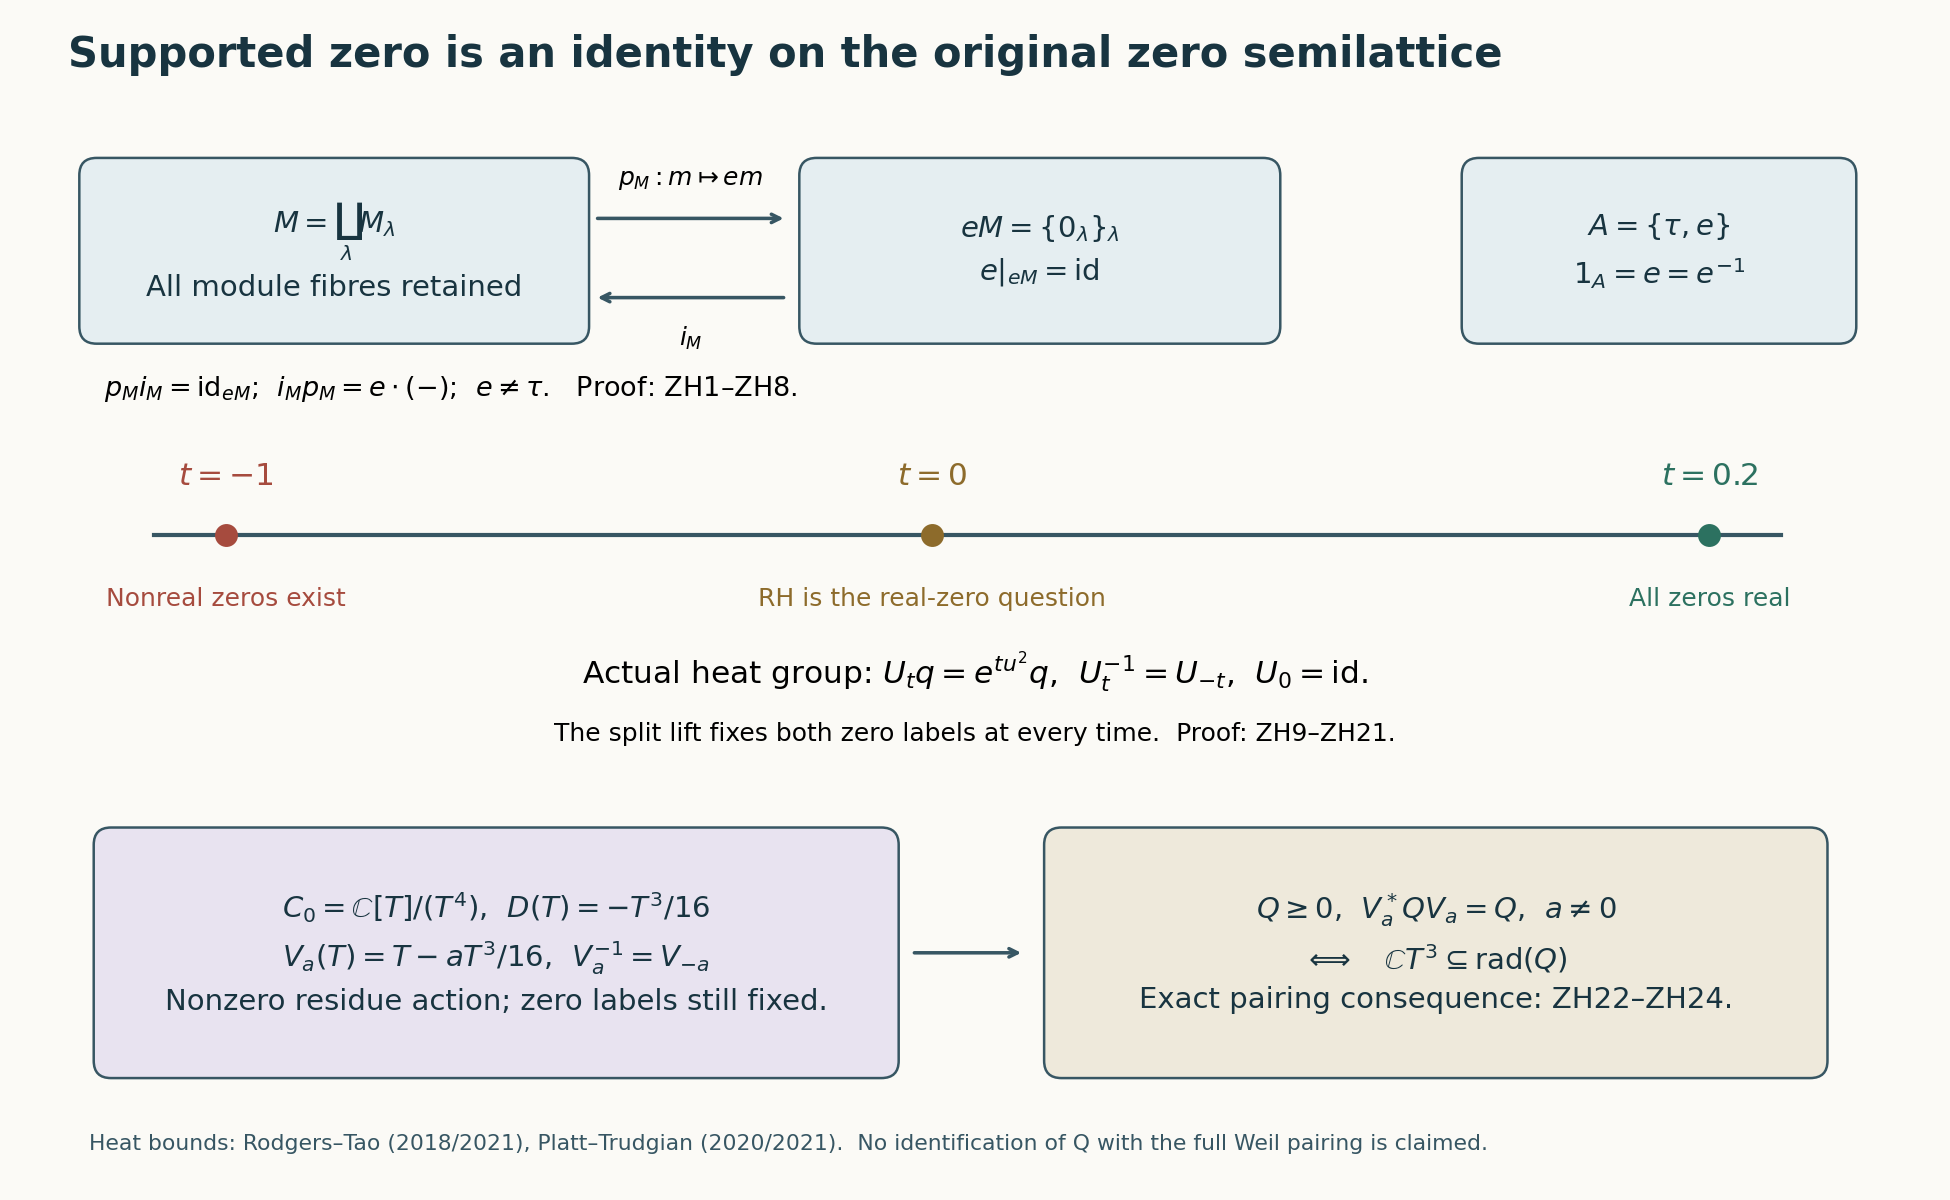
\includegraphics[keepaspectratio,alt={The original zero-semimodule retraction, the actual invertible heat evolution and its two known root regimes, and the exact invariant-form consequence of the retained residue. ZH1--ZH26 prove the displayed maps and statements. Time-marker positions are schematic and are not a numerical scale.}]{supported_zero_heat_identity.png}}
\caption{The original zero-semimodule retraction, the actual invertible
heat evolution and its two known root regimes, and the exact
invariant-form consequence of the retained residue. ZH1--ZH26 prove the
displayed maps and statements. Time-marker positions are schematic and
are not a numerical scale.}
\end{figure}

The reproducible figure source is
draw\_supported\_zero\_heat\_identity.py; both its PNG and SVG are
retained. The PNG was visually inspected. The two arrows at the top
preserve all module fibres and support labels; the lower arrow concerns
the residue-generated action, with no identification with an arithmetic
Weil pairing assumed.

\end{document}
